
%
% foundations - mapping
%

\section{Web Mapping}

Maps have become an almost instinctive way of seeing our world. They probably first appeared over 18,000 years ago and already in the 1500s, they were produced in large numbers for navigational and military purposes. Maps are powerful tools that help organize boundaries and administrative activities. They allow telling stories, visualizing data and understanding geographic contexts
~\cite{Zzolo11mappingdrupal}.

Recently, Google Maps\footnote{\url{http://maps.google.com}} has made digital maps available to a large number of internet users. Digital natives are used to navigate using interactive maps on their smart phones and look up places on online maps on their computers.

Web mapping describes the whole process of designing, implementing, generating and delivering maps on the internet. It applies theoretical foundations from web cartography to the technical possibilities and boundaries of constantly evolving web technologies. The continuous development of related technologies has created a wide variety of \textit{types of web maps}: from analytic, animated, collaborative and dynamically created web maps to online atlases, realtime and static web maps~\cite{wiki:web-mapping}.

\subsection{Map Projections}

The planet earth is a roughly spherical geoid. In order to represent it on flat computer screens, the surface of the earth needs to be translated to a plane. This is realized by applying the method of a map projection. Choosing a map projection influences how shapes, areas, directions and distances will be preserved or distorted. As no projection can optimize all those factors at once, choosing the right projection depends on the purpose of the map.

The \textit{spherical mercator projection} is the most commonly used web mapping projection. It preserves shapes and direction, but does this at the cost of enlarging areas towards the poles. This distortion can be visualized by Tissot's indicatrix. Figure \ref{fig:mercator} shows how circles of the same relative size get extrapolated off the equator by using the mercator projection~\cite{Zzolo11mappingdrupal, wiki:web-mapping}. 

\begin{figure}[h]
  \begin{center}
    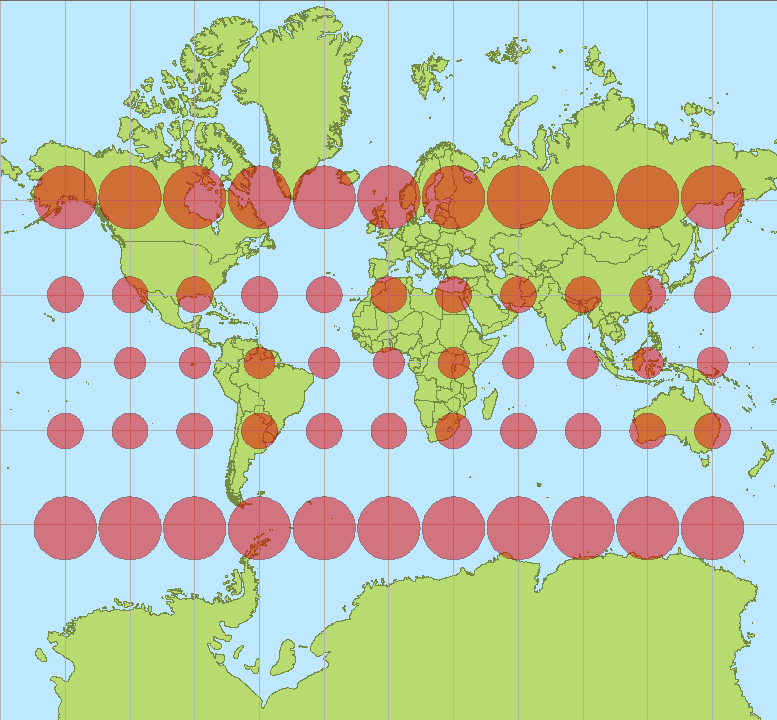
\includegraphics[width=0.5\textwidth]{figures/tissot_mercator.png}
    \label{fig:mercator}
    \caption{Tissot's indicatrix visualizes enlarged areas towards the poles when using the mercator projection~\cite{wiki:mercator}.}
  \end{center}
\end{figure}
   




























